\section{Frames and Bases}\label{sec:part1}

\begin{enumerate}[(a)]
\item The synthesis operator associated with $\{\varphi_k\}_{k \in \mathcal{K}}$ in $\mathbb{R}^2$ is
\[\Phi\alpha = \sum_{k \in \mathcal{K}} \alpha_k \varphi_k\]
Hence,
\begin{align*}
	\Phi_1 &= \begin{bmatrix}
	\frac{1}{2} & 0\\
	\frac{\sqrt{3}}{2} & 1
	\end{bmatrix} \\
	\Phi_2 &= \begin{bmatrix}
	\frac{1}{2\sqrt{2}} & -\frac{\sqrt{3}}{\sqrt{2}} & \frac{1}{\sqrt{2}} & 0\\
	\frac{\sqrt{3}}{\sqrt{2}} & \frac{1}{2\sqrt{2}} & 0 & \frac{1}{\sqrt{2}}
	\end{bmatrix} \\
	\Phi_3 &= \begin{bmatrix}
	\frac{1}{2} & -\frac{\sqrt{3}}{2} \\
	\frac{\sqrt{3}}{2} & \frac{1}{2}
	\end{bmatrix} \\
	\Phi_4 &= \begin{bmatrix}
	1 & \frac{1}{\sqrt{2}} & 0 \\
	0 & \frac{1}{\sqrt{2}} & 1
	\end{bmatrix}
\end{align*}
(Note that we reuse the notation $\Phi$ to represent the matrix representation.)

\item For $\Phi \in \mathbb{R}^{M \times N}$, if $M = N$ then it is a basis, if $M > N$ then it is a frame. 


Let $A$ be the inverse of the Gram matrix of basis $\Phi$, i.e. $A = (\Phi^* \Phi)^{-1}$. Then $\title{\Phi} = \Phi A = \Phi (\Phi^* \Phi)^{-1}$ forms a dual basis with $\Phi$.

Let $B = (\Phi \Phi^*)^{-1}$ , where $\Phi$ is a frame. Then $\tilde{\Phi} = B \Phi = (\Phi \Phi^*)^{-1} \Phi$ forms the canonical dual frame associated with frame $\Phi$.

For $\Phi_1$ (basis),
\begin{align*}
	A_1 &= \begin{bmatrix}
	1 & \frac{\sqrt{3}}{2} \\
	\frac{\sqrt{3}}{2} & 1
	\end{bmatrix} \Rightarrow A_1^{-1} = \begin{bmatrix}
	4 & -2\sqrt{3} \\
	-2\sqrt{3} & 4
	\end{bmatrix} \\
	\tilde{\Phi}_1 &= \begin{bmatrix}
	2 & -\sqrt{3} \\
	0 & 1
	\end{bmatrix}
\end{align*}

For $\Phi_2$ (frame),
\begin{align*}
	B_2 &= \frac{1}{2} \begin{bmatrix}
	\frac{1}{2} & -\frac{\sqrt{3}}{2} & 1 & 0 \\
	\frac{\sqrt{3}}{2} & \frac{1}{2} & 0 & 1
	\end{bmatrix} \begin{bmatrix}
	\frac{1}{2} & \frac{\sqrt{3}}{2} \\
	-\frac{\sqrt{3}}{2} & \frac{1}{2} \\
	1 & 0\\
	0 & 1
	\end{bmatrix}= \begin{bmatrix}
	1 & 0 \\
	0 & 1
	\end{bmatrix} = B_2^{-1} \\
	\tilde{\Phi}_2 &= \frac{1}{\sqrt{2}}\begin{bmatrix}
	1 & 0 \\
	0 & 1
	\end{bmatrix} \begin{bmatrix}
	\frac{1}{2} & -\frac{\sqrt{3}}{2} & 1 & 0 \\
	\frac{\sqrt{3}}{2} & \frac{1}{2} & 0 & 1
	\end{bmatrix} = \frac{1}{\sqrt{2}} \begin{bmatrix}
	\frac{1}{2} & -\frac{\sqrt{3}}{2} & 1 & 0 \\
	\frac{\sqrt{3}}{2} & \frac{1}{2} & 0 & 1
	\end{bmatrix} = \Phi_2
\end{align*}

For $\Phi_3$ (basis),
\begin{align*}
	A_3 &= \frac{1}{4}\begin{bmatrix}
	1 & \sqrt{3} \\ -\sqrt{3} & 1
	\end{bmatrix} \begin{bmatrix}
	1 & -\sqrt{3} \\ \sqrt{3} & 1
	\end{bmatrix} = \begin{bmatrix}
	1 & 0 \\ 0 & 1
	\end{bmatrix} = A_3^{-1} \\
	\Rightarrow \tilde{\Phi}_3 &= \Phi_3
\end{align*}

For $\Phi_4$ (basis),
\begin{align*}
	B_4 &= \begin{bmatrix}
	\frac{3}{2} & \frac{1}{2} \\
	\frac{1}{2} & \frac{3}{2}
	\end{bmatrix} \Rightarrow B_4^{-1} = \begin{bmatrix}
	\frac{3}{4} & -\frac{1}{4} \\
	-\frac{1}{4} & \frac{3}{4}
	\end{bmatrix} \\
	\tilde{\Phi}_4 &= \begin{bmatrix}
	\frac{3}{4} & \frac{1}{2\sqrt{2}} & -\frac{1}{4} \\
	-\frac{1}{4} & \frac{1}{2\sqrt{2}} & \frac{3}{4}
	\end{bmatrix}
\end{align*}

Figure \ref{fig:set_dual} shows the sketch of the sets and their duals.

\begin{figure}[htbp]
	\centering
	\begin{subfigure}[b]{0.49\textwidth}
		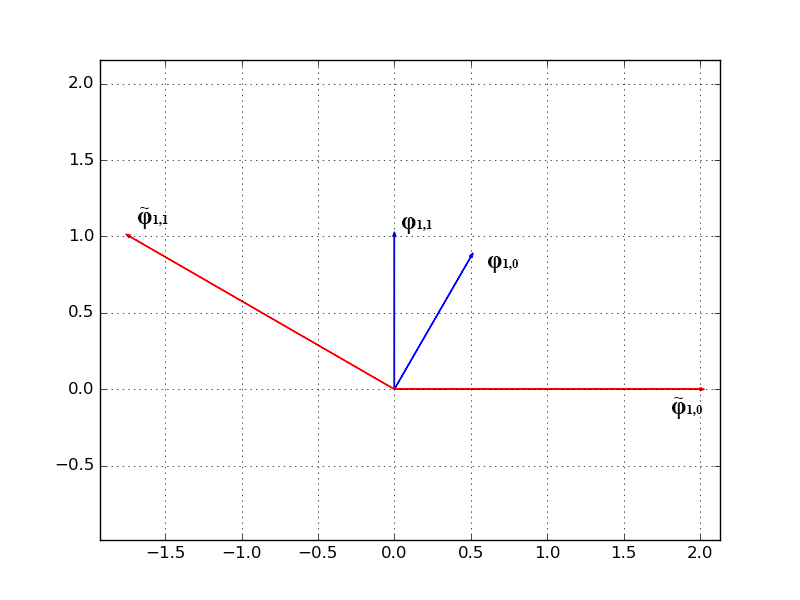
\includegraphics[width=\textwidth,trim={0.5in 0.5in 0.5in 0.5in},clip]{images/phi1}
		\caption{$\Phi_1$}
	\end{subfigure}
	\begin{subfigure}[b]{0.49\textwidth}
		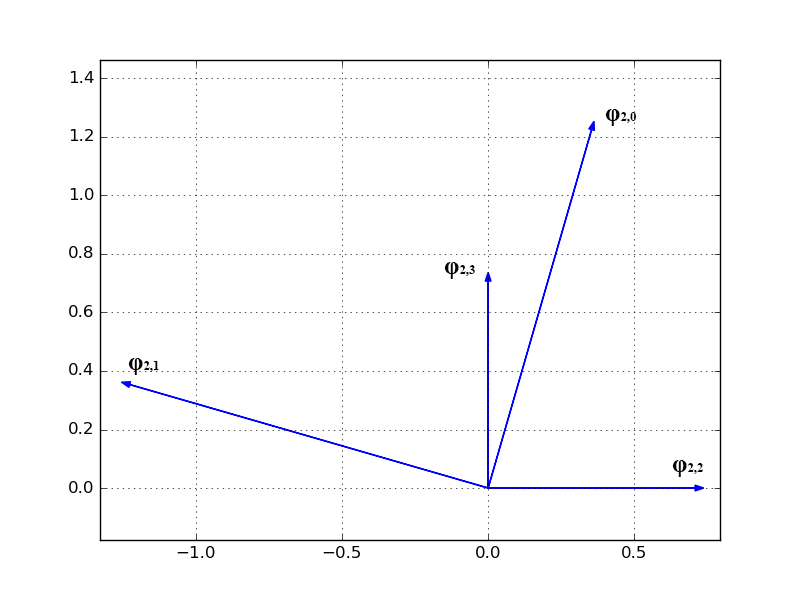
\includegraphics[width=\textwidth,trim={0.5in 0.5in 0.5in 0.5in},clip]{images/phi2}
		\caption{$\Phi_2$}
	\end{subfigure}
	\\
	\begin{subfigure}[b]{0.49\textwidth}
		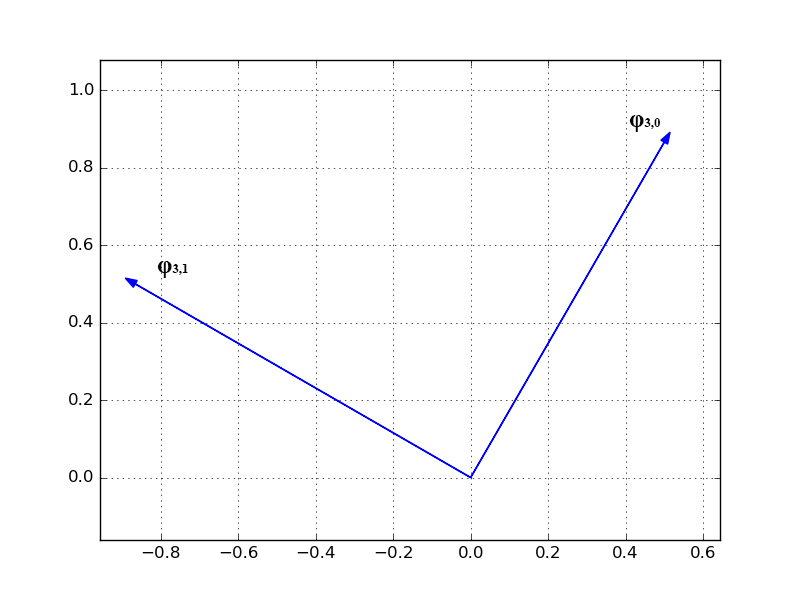
\includegraphics[width=\textwidth,trim={0.5in 0.5in 0.5in 0.5in},clip]{images/phi3}
		\caption{$\Phi_3$}
	\end{subfigure}
	\begin{subfigure}[b]{0.49\textwidth}
		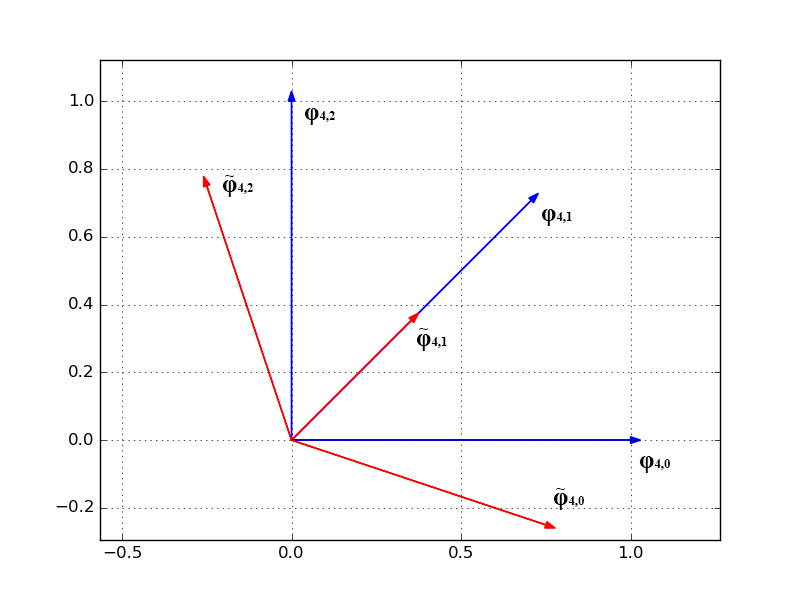
\includegraphics[width=\textwidth,trim={0.5in 0.5in 0.5in 0.5in},clip]{images/phi4}
		\caption{$\Phi_4$}
	\end{subfigure}
	\caption{Original sets and their duals.}\label{fig:set_dual}
\end{figure}

\item $\innerprod{\varphi_{1,0}}{\varphi_{1,1}} = \frac{\sqrt{3}}{2}$, so the basis $\Phi_1$ is not orthogonal, thus not orthonormal. $B_2 = I$, so the frame $\Phi_2$ is tight (a frame is tight if $\Phi \Phi^* = I$.) $\innerprod{\varphi_{3,0}}{\varphi_{3,1}} = 0$ and $\norm{\varphi_{3,0}} = \norm{\varphi_{3,1}} = 1$, so the basis $\Phi_3$ is orthonormal. $B_4 \neq I$, so the frame $\Phi_4$ is not tight.

\item $x = \begin{bmatrix}2 \\ 0\end{bmatrix}$ and $\alpha_{i,k} = \innerprod{x}{\tilde{\varphi}_{i,k}}$. Therefore,

For $\Phi_1$,
\begin{align*}
	&\alpha_{1,0} = \innerprod{\vect{2\\0}}{\vect{2\\0}} = 4
	&\alpha_{1,1} = \innerprod{\vect{2\\0}}{\vect{-\sqrt{3}\\1}} = -2\sqrt{3}
\end{align*}

For $\Phi_2$,
\begin{align*}
	&\alpha_{2,0} = \frac{1}{\sqrt{2}}\innerprod{\vect{2\\0}}{\vect{\frac{1}{2}\\\frac{\sqrt{3}}{2}}} = \frac{1}{\sqrt{2}}
	&\alpha_{2,1} = \frac{1}{\sqrt{2}}\innerprod{\vect{2\\0}}{\vect{-\frac{\sqrt{3}}{2} \\ \frac{1}{2}}} = -\sqrt{\frac{3}{2}} \\
	&\alpha_{2,2} = \frac{1}{\sqrt{2}}\innerprod{\vect{2\\0}}{\vect{1\\0}} =  \frac{2}{\sqrt{2}}
	&\alpha_{2,3} = \frac{1}{\sqrt{2}}\innerprod{\vect{2\\0}}{\vect{0\\1}} = 0
\end{align*}

For $\Phi_3$,
\begin{align*}
	&\alpha_{3,0} = \frac{1}{2}\innerprod{\vect{2\\0}}{\vect{1\\\sqrt{3}}} = 1
	&\alpha_{3,1} = \frac{1}{2}\innerprod{\vect{2\\0}}{\vect{-\sqrt{3}\\1}} = -\sqrt{3}
\end{align*}

For $\Phi_4$,
\begin{align*}
	&\alpha_{4,0} = \innerprod{\vect{2\\0}}{\vect{\frac{3}{4}\\-\frac{1}{4}}} = \frac{3}{2}
	&\alpha_{4,1} = \frac{1}{2\sqrt{2}}\innerprod{\vect{2\\0}}{\vect{1\\1}} = \frac{1}{\sqrt{2}}\\
	&\alpha_{4,2} = \innerprod{\vect{2\\0}}{\vect{-\frac{1}{4}\\ \frac{3}{4}}} = -\frac{1}{2}
\end{align*}

\item We check the values for $\alpha_{i,k}$ by verifying the expansion $x = \sum_k \alpha_{i,k} \varphi_{i,k}.$

For $\Phi_1$,
\[\sum_{k} \alpha_{1,k}\varphi_{1,k} = 4\vect{\frac{1}{2} \\ \frac{\sqrt{3}}{2}} - 2\sqrt{3}\vect{0 \\ 1} = \vect{2 \\ 0} = x\]

For $\Phi_2$,
\[\sum_{k} \alpha_{2,k}\varphi_{2,k} = \frac{1}{2}\left(1\vect{\frac{1}{2}\\\frac{\sqrt{3}}{2}} -\sqrt{3}\vect{-\frac{\sqrt{3}}{2} \\ \frac{1}{2}} +2\vect{1 \\ 0}\right) = \vect{2\\0} = x\]

For $\Phi_3$,
\[\sum_{k} \alpha_{3,k}\varphi_{3,k} = \vect{\frac{1}{2} \\ \frac{\sqrt{3}}{2}} - \sqrt{3}\vect{-\frac{\sqrt{3}}{2} \\ \frac{1}{2}} = \vect{2 \\ 0} = x\]

For $\Phi_4$,
\[\sum_{k} \alpha_{4,k}\varphi_{4,k} = \frac{3}{2}\vect{1 \\ 0} + \frac{1}{\sqrt{2}}\vect{\frac{1}{\sqrt{2}}\\\frac{1}{\sqrt{2}}} -\frac{1}{2}\vect{0\\1} = x\]

\item We verify that $\Phi \tilde{\Phi}^\top = I$.
\[\Phi_1 \tilde{\Phi}_1^\top = \begin{bmatrix}\frac{1}{2} & 0\\\frac{\sqrt{3}}{2} & 1\end{bmatrix}\begin{bmatrix}2 & 0 \\ -\sqrt{3} & 1\end{bmatrix} = I\]

\[\Phi_2 \tilde{\Phi}_2^\top = \Phi_2 \Phi_2^\top = B_2 = I\]

\[\Phi_3 \tilde{\Phi}_3^\top = \Phi_3 \Phi_3^\top = \begin{bmatrix}\frac{1}{2} & -\frac{\sqrt{3}}{2} \\ \frac{\sqrt{3}}{2} & \frac{1}{2}\end{bmatrix} \begin{bmatrix}\frac{1}{2} & \frac{\sqrt{3}}{2} \\ -\frac{\sqrt{3}}{2} & \frac{1}{2}\end{bmatrix} = I\]

\[\Phi_4 \tilde{\Phi}_4^\top = \begin{bmatrix}1 & \frac{1}{\sqrt{2}} & 0 \\ 0 & \frac{1}{\sqrt{2}} & 1\end{bmatrix} \begin{bmatrix} \frac{3}{4} & -\frac{1}{4} \\ \frac{1}{2\sqrt{2}} & \frac{1}{2\sqrt{2}} \\ -\frac{1}{4} & \frac{3}{4} \end{bmatrix} = I\]

\item We check if $\norm{x}^2 = \sum_k\abs{\alpha_{i,k}}^2$.
\[\norm{x}^2 = \norm{\vect{2\\0}}^2 = 4^2 = 16\]

\[\sum_k\abs{\alpha_{1,k}}^2 = 28\]

\[\sum_k\abs{\alpha_{2,k}}^2 = \frac{13}{4}\]

\[\sum_k\abs{\alpha_{3,k}}^2 = 4\]

\[\sum_k\abs{\alpha_{4,k}}^2 = 3\]

Hence, the expansion does not preserve the norm.

\item Since all of the expansion $\sum_k \alpha_{i,k} \varphi_{i,k} = x$, the expansion is redundant.
\end{enumerate}